\chapter{Short Baseline Neutrino Program}
\label{chp:sbn}

This chapter will describe the Short Baseline Neutrino Program, and the anomalies it is seeking to resolve.

\section{Motivation and Goals}

Over the past two decades, experimental hints of beyond the Standard Model neutrino physics have appeared in several distinct subfields of neutrino experiments.  Taken together, the constitute hints at oscillation physics on mass splitting scale that is inconsistent with the known oscillations models.  This section will briefly summarize the current anomalies in this area of neutrino oscillations, known as Short Baseline oscillation physics.

A more thorough analysis of the global, experimental picture of neutrino oscillations is given by oscillation analyses such as Kopp et. al \cite{Kopp:2013vaa}, Giunti et. al \cite{Giunti:2013aea}.  Though there is tension in the experimental evidence, there is indication that anomalous neutrino oscillation is occurring at short baselines.


\subsection{LSND}

In 1995, the Liquid Scintillator Neutrino Detector at Los Alamos National Laboratory published the results of it's first search for \numubar to \nuebar oscillations \cite{Athanassopoulos:1995iw}.  The detector was a liquid scintillator detector making observations of electron anti neutrinos through the inverse beta decay reaction on carbon.  The origin of the neutrinos was a decay at rest pion source, producing neutrinos in the range of 20 to 50 MeV.  In the inverse beta decay reaction signature is a prompt positron emission, followed by a 2.2 MeV gamma from neutron capture.   LSND observed 89.7 $\pm$ 22.4 $\pm$ 6.0 \nuebar candidate events above background over five years of data taking, corresponding to a significance of 3.8 $\sigma$.


\begin{figure}[htbp]
    \centering
    \begin{subfigure}[t]{0.5\textwidth}
        \centering
        \includegraphics[height=3in]{sbn_figures/lsnd_beam_excess}
    \end{subfigure}%
    ~ 
    \begin{subfigure}[t]{0.5\textwidth}
        \centering
        \includegraphics[height=3in]{sbn_figures/lsnd_allowed_region_by_lsnd.pdf}
    \end{subfigure}
    \caption[LSND Excess]{ (Left) Excess of candidate \nuebar events observed by LSND, plotted as a function of L/E of the reconstructed neutrino. (Right) Allowed region of oscillation parameters when fit against a 2 neutrino mixing model.}
   \label{fig:lsnd_beam_excess}
\end{figure}

As seen in Figure~\ref{fig:lsnd_beam_excess}, the LSND excess is inconsistent with the three neutrino oscillation paradigm.  Instead, it hints at oscillations at L/E of $\sim$ 0.5 and a mass splitting of $\sim$ 1 eV$^2$.  For comparison, the  solar and atmospheric mass splittings are in the ranges of $7\times10^{-5}\text{ eV~}^2$ and $2\times10^{-2}\text{ eV~}^2$, respectively.

\subsection{Reactor Experiments}

Many experiments have measured the flux of neutrinos from nuclear reactors over many years.  However, a recent reevaluation \cite{Huber:2011wv} \cite{Mueller:2011nm} of the expected neutrino flux from reactors has led to an observed deficit in historical measurements, as seen in Figure~\ref{fig:reactor_deficit} \cite{Mention:2011rk}.  This deficit, at the level of 6 to 7\%, is consistent with an oscillation of reaction \nuebar into an unobserved sterile state.

Some concern over the so called Reactor Deficit has been raised over the fact that before the recalculation was completed, all experiments were in agreement with the existing theoretical prediction.  However, experimental results from the Daya Bay collaboration \cite{An:2015nua}, done in a blind analysis, support the experimental evidence of the reactor neutrino deficit (See Figure~\ref{fig:daya_bay_reactor_flux}).

\begin{figure}[htbp]
  \centering
  \includegraphics[width=\textwidth]{sbn_figures/reactor_flux.pdf}
  \caption[Reactor Deficit]{Measurements of the reactor neutrino flux indicate a deficit when compared with theoretical predictions.  It's plausible that the deficit is evidence of anomalous neutrino oscillations.}
  \label{fig:reactor_deficit}
\end{figure}

\begin{figure}[htbp]
  \centering
  \includegraphics[]{sbn_figures/daya_bay_flux_deficit.pdf}
  \caption[Daya Bay Reactor Flux]{The Daya Bay experiment performed a blind measurement of the reactor flux and their location and found excellent agreement with previous experimental data.  This was performed after the flux recalculations.}
  \label{fig:daya_bay_reactor_flux}
\end{figure}

% \subsection{Source Experiments}

% For measurement of Solar Neutrinos, the experiments GALLEX and SAGE both used radioactive sources as a neutrino source for calibration.

% \cite{Abdurashitov:1998ne} \cite{Hampel:1997fc}

\subsection{\label{sec:miniboone} \MB}

Most recently, the \MB collaboration published evidence for an excess of electron neutrino candidate events in both neutrino and anti neutrino mode at Fermilab's Booster Neutrino Beam \cite{Aguilar-Arevalo:2013pmq}.  Their results, shown in Figure~\ref{fig:mb_stacked_rates}, clearly indicate an excess of candidate events.  Despite the significance of the results (3.4 $\sigma$ for Neutrino Mode, 2.8 $\sigma$ in Anti-Neutrino Mode), the \MB results are particularly controversial.

First, the detector technology of \MB is a Cherenkov type detector, meaning that it distinguishes particles based upon their Cherenkov signature observed by PMTs at the outer surface of the detector.  Since electrons and photons both produce similar electromagnetic cascades, \MB is unable to distinguish between electron and photon events.  For the electron neutrino analysis in Figure~\ref{fig:mb_stacked_rates}, this implies that the excess can not be attributed as electron neutrinos without further investigation, and therefore isn't conclusively inconsistent with the standard three neutrino oscillation model.  It's worth mentioning, however, that the excess is significant enough to warrant \uboone's investigation, discussed in detail below.

Second, the \MB oscillation result is inconsistent with anticipated 3+1 model sterile neutrino oscillation signals.  As seen in Figure~\ref{fig:mb_stacked_rates}, the observed excess can not simultaneously be interpreted as electron neutrinos from muon neutrino oscillations (through a sterile state) while agreeing with the sterile neutrino oscillation model.

Despite the controversy, when taken with consideration into consideration with other results such as LSND (at the same L/E as \MB), and the reactor and source anomalies, there is intriguing evidence of physics beyond the Standard Model in the neutrino sector.


\begin{figure}[htbp]
  \centering
  \includegraphics[]{sbn_figures/miniboone_beam_excess.pdf}
  \caption[\MB Beam Excess]{Caption here}
  \label{fig:mb_beam_excess}
\end{figure}

\begin{figure}[htbp]
  \centering
  \includegraphics[]{sbn_figures/miniboone_stacked_rates.pdf}
  \caption[\MB Stacked Rates]{Caption here}
  \label{fig:mb_stacked_rates}
\end{figure}

\subsection{Global Fits}
\label{sec:global_fits}

With many hints at beyond the standard model neutrino oscillations, analyses have been performed to bring together the various hints (and null results) in an attempt to constrain allowed phase space in sterile neutrino oscillations.  In particular, a viable explanation of the anomalies using sterile neutrinos must be in agreement across multiple signatures of oscillations, for a 3+1 model.  Ignoring CP violating terms (which are not observable in short baseline experiments), the mixing matrix for a 3+1 model is given as:

\begin{equation*}
\mathbf{U} = \left(
\begin{array}{cccc}
U_{e1} & U_{e2} & U_{e3} & U_{e4}  \\
U_{\mu1} & U_{\mu2} & U_{\mu3} & U_{\mu4}  \\
U_{\tau1} & U_{\tau2} & U_{\tau3} & U_{\tau4}  \\
U_{s1} & U_{s2} & U_{s3} & U_{s4}  \\
\end{array} \right)
\end{equation*}

\begin{enumerate}
  \item{ \em Electron Neutrino Disappearance:} An electron neutrino can oscillation into an unobservable, sterile neutrino state with amplitude given as
  \begin{align}
  P(\nue \rightarrow \nu_{\cancel{e}}) &\approx sin^2(2 \theta_{ee})\times sin(1.27 \frac{\Delta m^2 L}{E} \frac{[eV^2][m]}{[MeV]})),
   \\
  sin^2(2 \theta_{ee}) &\equiv 4 |U_{e4}|^2 (1 - |U_{e4}|^2) \approx 4 |U_{e4}|^2.
  \end{align}
  This is the oscillation regime that governs, for example, the reactor neutrino anomaly.
  \item { \em Muon Neutrino Disappearance: } In a nearly identical fashion as above, a muon type neutrino can oscillate into a sterile stage with amplitude 
  \begin{align}
  P(\numu \rightarrow \nu_{\cancel{\mu}}) &= sin^2(2 \theta_{\mu\mu})\times sin(1.27 \frac{\Delta m^2 L}{E} \frac{[eV^2][m]}{[MeV]})),
   \\
  sin^2(2 \theta_{\mu\mu}) &\equiv 4 |U_{\mu4}|^2 (1 - |U_{\mu4}|^2) \approx 4 |U_{\mu 4}|^2.
  \end{align}
  Intriguingly, there has been no observed signal of muon neutrino disappearance consistent with the same anomalies that hint towards sterile neutrino oscillations, despite searches by MINOS \cite{Adamson:2010wi}, \MB+SciBooNE \cite{Mahn:2011ea}, and IceCube \cite{TheIceCube:2016oqi}.

  \item { \em Electron (and Anti-Electron) Appearance:} Given that a sterile neutrino can have mixing parameter that connect to both electron and muon type neutrinos, it is possible to have an oscillation of muon neutrinos into electron neutrinos.
  \begin{align}
  P(\numu \rightarrow \nue) &= sin^2(2 \theta_{\mu e})\times sin(1.27 \frac{\Delta m^2 L}{E} \frac{[eV^2][m]}{[MeV]})),
   \\
  sin^2(2 \theta_{\mu e}) &\equiv 4 |U_{\mu4}|^2|U_{e4}|^2 \approx \frac{1}{4} sin^2(2 \theta_{ee}) sin^2(2 \theta_{\mu \mu}).
  \end{align}
  As seen in \cite{Kopp:2013vaa,Giunti:2011gz}, limits on the oscillation amplitude from electron neutrino and muon neutrino disappearance can place upper bounds on the amplitude of muon to electron neutrino oscillation.
\end{enumerate}

Taken together, the global data can be combined as in \cite{Kopp:2013vaa,Giunti:2011gz}.  In the best fit by Kopp et. al, there is no strongly allowed region though the tension between signals and null results is high.  In the best fit by Giunti et. al, there is an allowed region though the \MB anomaly is not included in this fit (for the inconsistencies mentioned above).


\section{FermiLab's Short Baseline Neutrino Program}

\label{sec:sbn_detectors}
With all of the above anomalies and hints of beyond the standard model, it is essential to address the sterile neutrino question and resolve the \MB anomaly.  To address these hints, Fermilab is pursuing a program of short baseline neutrino experiments along it's Booster Neutrino Beam.  The first experiment, \uboone, started operations in 2015 and is designed to definitively lay to rest the \MB anomaly.  Subsequently, two other detectors will join \uboone along the Booster Beam at 100m and 660m.  An overview of the three \lartpcs involved in Fermilab's Short Baseline Program is given in Sections \ref{sec:microboone} and \ref{sec:future_tpcs}.  The location of the three detectors can be seen in Figure~\ref{fig:sbn_birdseyeview}.

\begin{figure}[htbp]
  \centering
  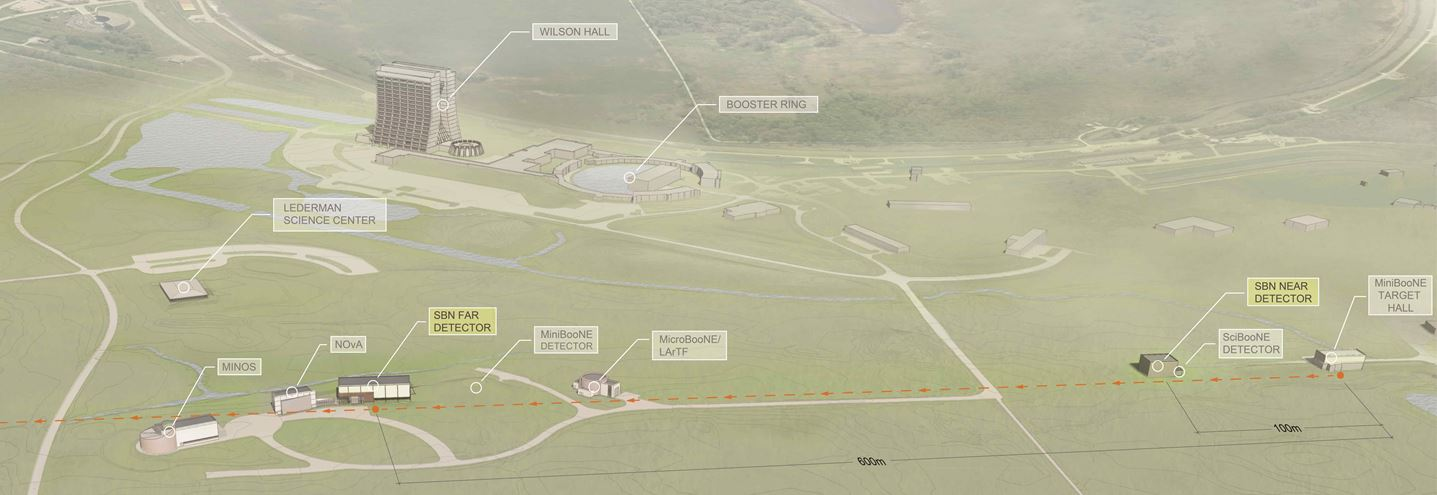
\includegraphics[width=\textwidth]{sbn_figures/SBN_Map.jpeg}
  \caption[SBN Detector Locations]{An aerial view of the SBN program.  The three detectors are highlighted in yellow, and (from right to left, along the path of the beam) are \sbnd, \uboone, and \icarus}
  \label{fig:sbn_birdseyeview}
\end{figure}

\section{Physics Program}

The Short Baseline Neutrino program has an aggressive agenda to probe anomalous oscillation signals, and to follow up on \uboone's Low Energy Excess analysis.  It's worth noting that \nue appearance is not the only physics analysis that will be performed by the SBN Program.  This thesis will focus on \nue appearance, however to resolve questions of sterile neutrinos the SBN program will also have to observe:

\begin{itemize}

\item {\bf \numu Disapperance}  As mentioned above, the channels of \nue appearance and \numu disappearance are intricately connected in models of sterile neutrino oscillations.  So, for any measurement of \nue appearance at the SBN Program to be interpreted in a 3+1 model of oscillations, it should be accompanied by an amount of \numu disappearance consistent with the level of \nue appearance.  Much more about \numu disappearance is available in the SBN Program Proposal \cite{Antonello:2015lea} 

\item {\bf Neutral Current Disappearance (Active flavor Disapperance)}  Just as the \nue and \numu oscillation signals are connected if a sterile neutrino is present, the total active flavor content of the beam (\nue + \numu + \nutau) should be modulated by the presence of a sterile neutrino in a consistent way.  \lartpc technology allows measurement of the total neutral current interaction rate using channels such as Neutral Current $\pi^0$ production.

\end{itemize}

Also of interest is the suite of cross section measurements that the SBN Program can perform, particularly with the SBND experiment (the near detector).  In the event that \uboone observes the \MB anomaly to be an unexpected beam background or cross section, SBND can probe this result with nearly two orders of magnitude faster collection of events than \uboone.

\section{Simulation and Monte Carlo Predictions of Event rates}

For the calculation and study of the physics sensitivity of the Short Baseline Program, a Monte Carlo Simulation predicts the event rate at each detector in the beamline.  The procedure of the simulation is:

\begin{enumerate}

  \item {\bf Booster Beam Monte Carlo} The first stage in the simulation is the Monte Carlo simulation of the Booster Neutrino Beam production. This is a geant4 based simulation that follows 8 GeV protons through interactions on the BNB beryllium target. The hadrons produced in the interaction are focus by the horn and decay, in flight, to neutrinos, which are then propagated to a window in front of a detector. It is at this stage of the simulation that we include a series of reweighting variables for each neutrino to estimate the systematic uncertainty on the flux at each detector, as well as the correlations between detectors (additional information in Section~\ref{section:flux_uncert}).

  \item {\bf \textsc{Genie} Neutrino Interactions} The output of the beam Monte Carlo is a file of neutrinos at the detector containing information about the flavor, momentum, and position, as well as the parentage from the beam source, for each neutrino. The interactions of these neutrinos are simulated with the genie software which outputs a series of particles exiting the argon nucleus \cite{Andreopoulos:2009rq}. 

  \item {\bf \textsc{Geant4} Simulation of Particles} The particles which exit the argon nucleus, as generated by genie, are then propagated through the liquid argon using a \textsc{Geant} \cite{Agostinelli:2002hh} simulation built in to the LArSoft framework \cite{Church:2013hea}. In particular this helps estimate the containment of electromagnetic showers, interaction location of photons from \pizero production and $\Delta$ resonances, as well as containment of minimally ionizing particles such as muons and charged pions.

  \item {\bf Monte Carlo Truth Based Information}  After the geant simulation of the neutrino interaction we extract the event information using the Monte Carlo truth information. Estimated reconstruction efficiencies and energy resolutions are applied at this stage, as well as simulated event selections based on expected detector performance.  See Section~\ref{subsection:event_reco} for more detail.

\end{enumerate}


\subsection{Background Classification}

For the study of the Short Baseline Neutrino Program's sensitivity to anomalous appearance of electron neutrinos, it is essential to have a comprehensive estimate of the various backgrounds with realistic distributions based on expected reconstruction ability.  Primarily, the \nue appearance background consists of 3 broad categories: intrinsic \nue's from the beam, mis-identified electromagnetic showers produced by the beam (primarily from \numu), and cosmic induced backgrounds coincidental with the beam spill.

\begin{enumerate}

  \item {\bf Intrinsic \nue } - the Booster Beam, while primarily composed of muon neutrinos, has contamination of electron neutrinos that account for about 0.5\% of the beam.  While this is a small contamination, it is the same order of magnitude as the best fit oscillation parameters for possible sterile neutrino hints. This means that, compared to any possible signal, the intrinsic electron neutrinos in the beam are a large background and must be carefully quantified.  An 80\% reconstruction efficiency is applied to these events, and an electromagnetic shower energy of 200MeV is set as a threshold for event selection.  This is to ensure good selection and reconstruction in the data, and has a moderate impact at lower energies on the efficiency (~30\% loss in the 200 to 350 MeV bin) with small impacts (~5\%) at higher energies.



  \item {\bf Neutral Current Photon Misidentification} - The photons produced in the detector by neutral current processes can produce an electromagnetic shower similar to electron neutrinos.  An example of a reaction that produces high energy photons is an interaction with neutral pions in the final state, as well as radiative decays from nucleon resonances. It's expected that, without cuts, these backgrounds can be large and in the same energy region as a signal search. However, analysis cuts can greatly reduce this background.

  \begin{enumerate}

    \item{\em Two photon cut:} In an event with candidate electromagnetic showers, the presence of multiple showers indicates there could be neutral pion production in the neutrino interaction.  See, for example, Figure~\ref{fig:argo_pi0} for an ArgoNeuT event with multiple showers.  For this analysis, if a second found is found with energy greater than 100 MeV, the event is rejected from the electron neutrino sample.  The energy cut, 100 MeV, is lower than the threshold for candidate electron showers because the second photon does not need accurate reconstruction, it just needs to be identified.

    \item{\em Photon Conversion Gap:} In events where the neutrino interaction produces high energy photons, it can at times also product hadronic activity at the vertex.  If more than 50 MeV of energy is observed at the vertex, and a gap between the electromagnetic shower and the vertex is detected with more than 3 centimeters (in \uboone, this is up to 30 wires), the event is rejected.

    \item{\em dE/dx Cut:} In this study, for events passing the previous two cuts, and 94\% rejection was applied.  This accounts for the expected resolution, in the SBN detectors, of the calorimetric based cut on the ionization of the first few centimeters of a shower.  For more about the power of the dE/dx cut in data, see Section~\ref{sec:argo_dedx}

  \end{enumerate}


  \item {\bf Neutrino Electron Scattering}  - neutrinos can scatter off both the nucleus and the orbiting electrons in an atom. An interaction off an electron ejects the electron at high energy. Experimentally, the signature of this interaction is a very forward going electron and nothing else in the event, which mimics a \nue charged current interaction. Fortunately, these events have a very low interaction rate compared to scattering off of a nucleus and are a secondary background.  The forward angle and relatively high energy also make them a removable background.

  \item {\bf \numu Charge Current Misidentification} - The last item considered as a possible background are misidentified charged current interactions from muon neutrinos. The rate at which this happens is poorly know and needs to be measured, but there are some scenarios that could lead to this occurring. For example, in an event near the boundary of the TPC where a \pizero is produced along with the primary muon, if the muon exits and one photon converts outside the TPC there will be one electromagnetic shower seen and the track of the muon will be impossible to tag as a muon or charged pion. Though somewhat contrived, this example only serves to illustrate that this background should be considered. Here, events are included from \numu CC interactions if there is a single photon in the detector and the primary muon exits with less than one meter in the detector.
  
  \item {\bf Cosmic Photons} - Cosmic induced photons in the TPC have the potential to be incorrectly tagged as electrons. This is a background that will be very tightly constrained from off-beam backgrounds, but estimates from simulation are included here.

  \item{\bf ``Dirt'' Events} - Neutrinos can interact with the material surrounding the active volume of the detector as well.  Though this is not, strictly speak, ``dirt'', events where detector external neutrino interactions travel into the TPC and deposit energy can cause a background to the \nue appearance analysis.  In particular, photon production external to the TPC can generate a high energy photon that travels into the TPC and doesn't ionize the argon until it has entered the TPC for some distance.  This background will be constrained with both simulation and data, however, preliminary estimates are included.  Additionally, strong cuts can be made with fiducial volumes.

\end{enumerate}

\begin{figure}[htbp]
  \centering
  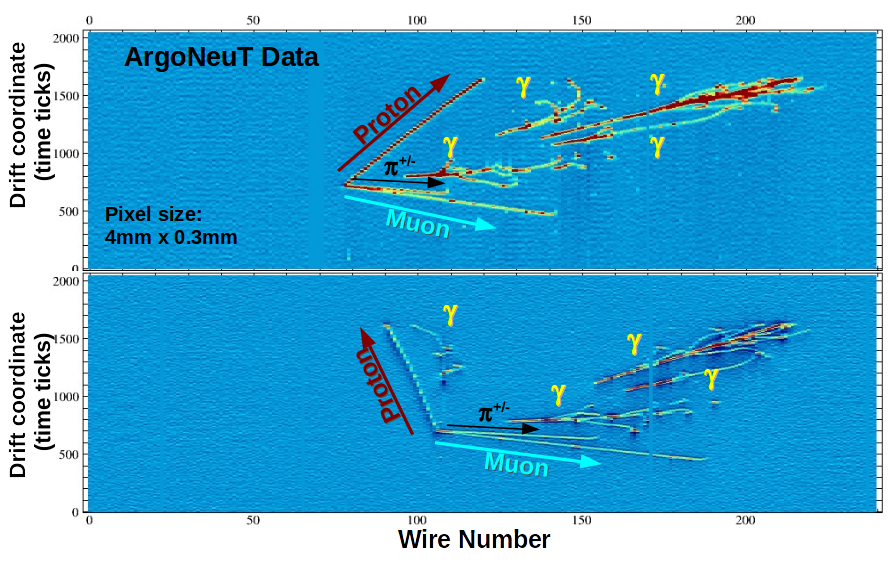
\includegraphics[width=0.95\textwidth]{sbn_figures/ArgoNeuT_Labels.png}
  \caption{caption}
  \label{fig:argo_pi0}
\end{figure}

\subsection{Simulated Event Reconstruction and Analysis cuts}
\label{subsection:event_reco}

In order to perform the best estimate of the physics sensitivity of the SBN program, an estimate of reconstruction effects must be incorporated into the event rates.  Additionally, some analysis cuts to reduce cosmic and ``dirt'' events are included.

The simplest cut is the fiducial volume cut applied in all three detectors.  Events with a vertex found to be outside of the fiducial volume are rejected, and the volume is set as:
\begin{itemize}
\item{\bf X:} The drift direction has a cut of 25cm from each edge, which reduces ``dirt'' backgrounds significantly.
\item{\bf Y:} The vertical direction also has a cut of 25cm from each edge, which reduces ``dirt'' backgrounds significantly.
\item{\bf Z:} The beam direction has an upstream cut of 30cm, to reject events that are entering the detector from the front.  There is a downstream cut of 50cm to aid in detection of electromagnetic showers.
\end{itemize}

To simulate calorimetric energy reconstruction, the incoming neutrino energy in each Monte Carlo event is estimated by summing the energy of the lepton (or the $\gamma$ the faking an electron) and all charged hadrons above observation thresholds present in the final state.  The observation thresholds are defined by requiring that the kinetic energy of each hadron be sufficient that it cross at least 2 wires, and are guided by \argoneut data.  For protons, for example, the threshold is 20 MeV. 

The event rate distributions, and the tables of event rates, are shown in Figure~\ref{fig:sbn_event_rates_no_signal} and sidewaysTable~\ref{tab:sbn_event_rates_no_signal}.

\begin{figure}[htbp]
    \centering
    \begin{subfigure}[]{0.49\textwidth}
        \centering
        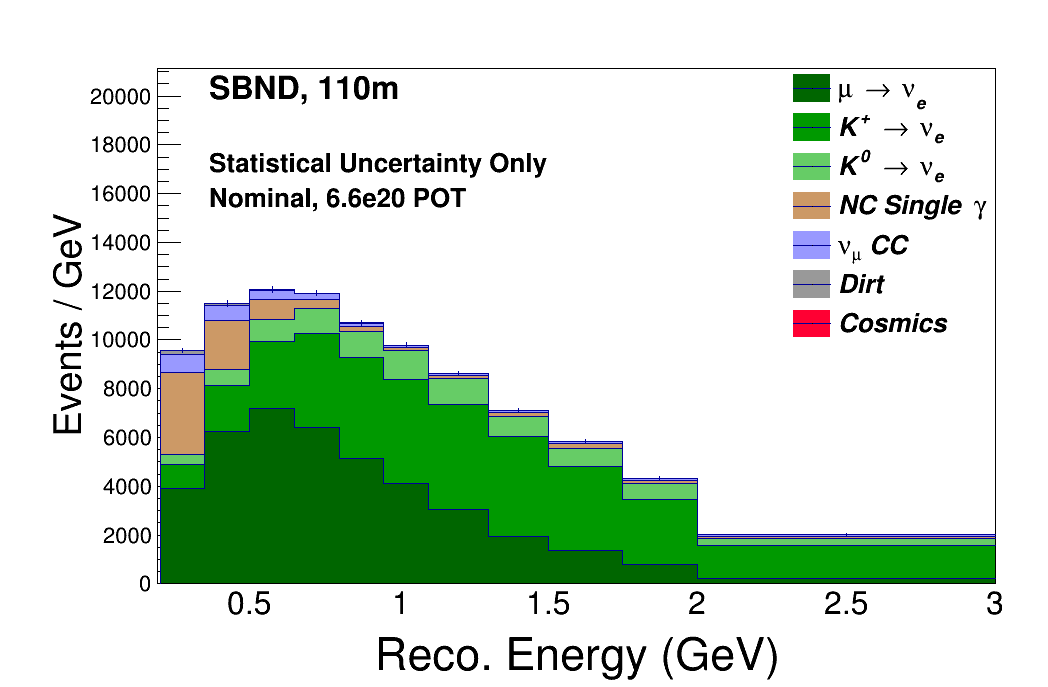
\includegraphics[width=\textwidth]{sbn_figures/nominal_nue_appearance_nosig_SBND_110m}
    \end{subfigure}
    ~
    \begin{subfigure}[]{0.49\textwidth}
        \centering
        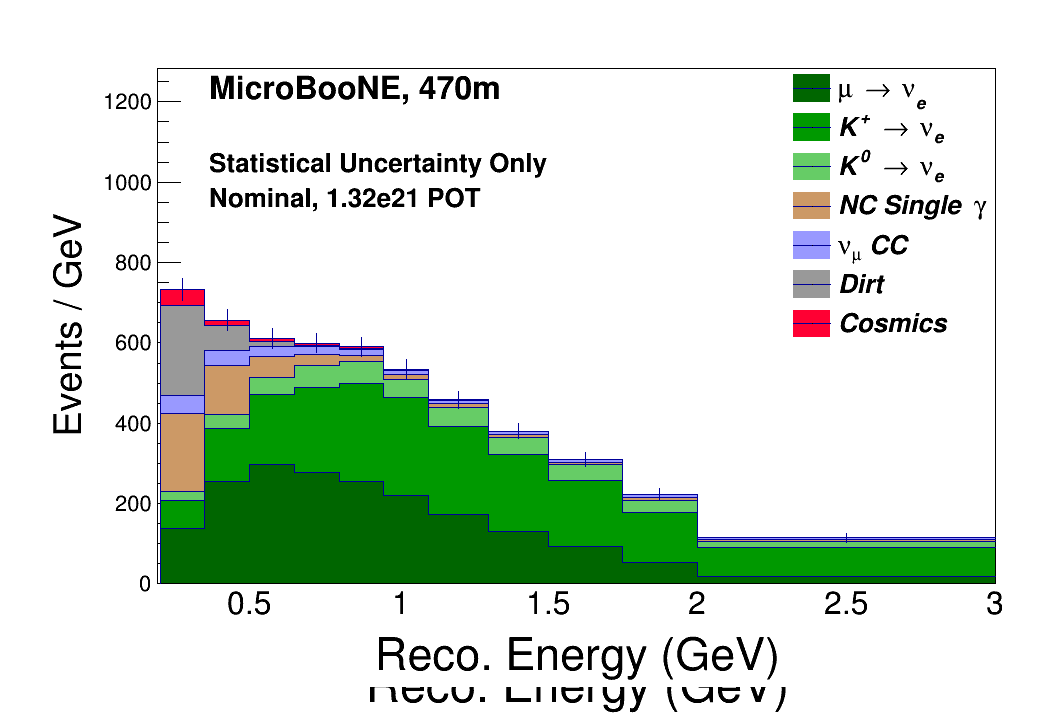
\includegraphics[width=\textwidth]{sbn_figures/nominal_nue_appearance_nosig_MicroBooNE_470m}
    \end{subfigure}
    \\
    \begin{subfigure}[]{0.49\textwidth}
        \centering
        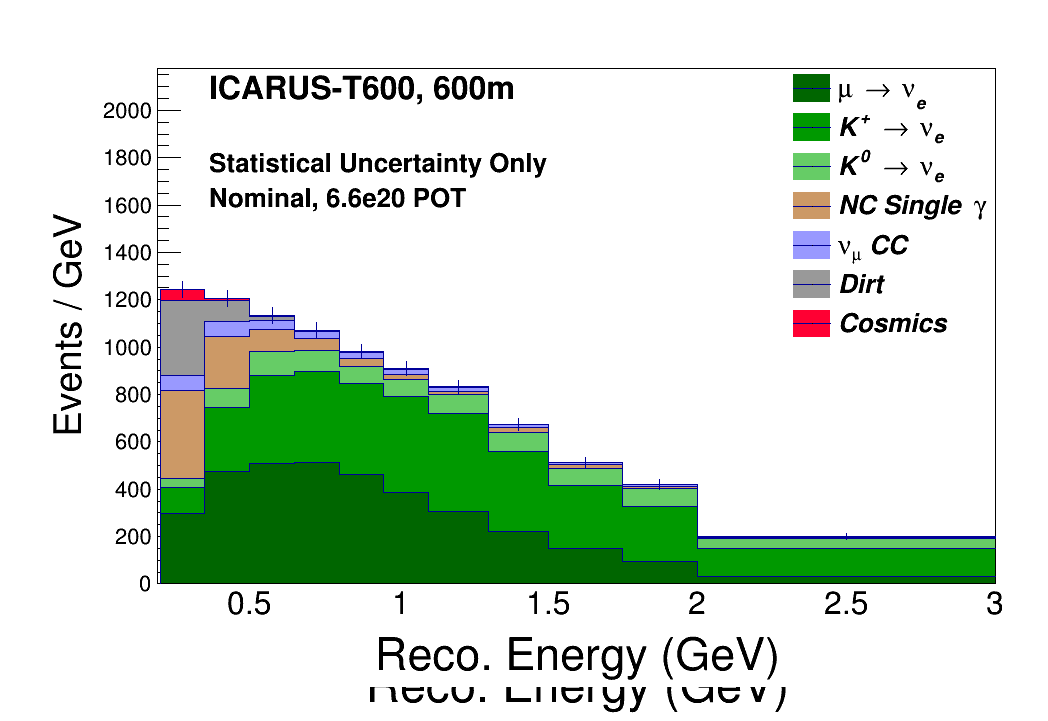
\includegraphics[width=\textwidth]{sbn_figures/nominal_nue_appearance_nosig_ICARUS-T600_600m}
    \end{subfigure}
    \caption[SBN Event Rates]{The predicted event rates for the SBN program in all three detectors, assuming 2.2e20 Protons on Target delivered each year.  For this analysis, \uboone is assumed to have 6 years of running (its original 3 + 3 with the SBN program)}.
   \label{fig:sbn_event_rates_no_signal}
\end{figure}

\section{Simulation of an Oscillation Signal}

To predict a sensitivity of an experimental program, a model must be used to generate a sample of events that are signal events.  In this case, as mentioned in Section~\ref{sec:global_fits}, the two neutrino oscillation probability formula is used to transmute muon neutrinos into electron neutrinos.  While the 3+1 model is not the only viable or interesting method to simulate a signal, it is the most straightforward to compare to other experiments.  

To build a signal sample, a ``fully oscillated'' sample of Monte Carlo is generated where every \numu has been changed to a \nue, and then the sample of \nue's is propagated through the GENIE event generator and the rest of the simulation.  Each electron neutrino, formerly muon neutrino, is ``reconstructed'' in the same manner as the electron neutrino candidates in the background sample, with identical cuts.  

Later, a sensitivity curve will be shown as a function of ($\Delta_m^2,\text{sin}^2 2 \theta$).  This refers to physical parameters of neutrino oscillation, where $\Delta m^2$ is the mass splitting, squared, between known neutrinos and a supposed sterile state.  Sin${}^2 2 \theta$ represents the amplitude of the oscillation and is a combination of matrix elements from the neutrino mixing matrix above.  For a fixed pair of ($\Delta_m^2,\text{sin}^2 2 \theta$), each transmuted electron neutrino in the ``fully oscillated'' sample is scaled according to the formula 

\begin{equation}
% \centering
P(\numu \rightarrow \nue) = sin^2(2 \theta_{\mu e})\times sin(1.27 \frac{\Delta m^2 L}{E} \frac{[eV^2][m]}{[MeV]})),
\end{equation}
where L and E are known from the Monte Carlo as the distance the neutrino has traveled since the decay of it's parent particle, and the true energy of the neutrino.  Because the neutrino beam is broad band, peaked near 1 GeV but with substantial flux down to several hundred MeV and out to 3 GeV, the oscillation probabilities at each detector are smeared and the predicted signal can cover a broad spectrum of neutrino energies (see Figure~\ref{fig:osc_prob} )
% tables were made with the help of http://www.tablesgenerator.com/

\begin{figure}[htbp]
  \centering
  \includegraphics[width=\textwidth]{sbn_figures/osc_prob.pdf}
  \caption[BNB Oscillation Probability]{Oscillation Probability bands as a function of distance from the proton target for the SBN program.  Shown are the bands for two of the global best fit results.}
  \label{fig:osc_prob}
\end{figure}


\begin{sidewaystable}[htbp]
\centering

\caption{Background Rates, broken out by analysis bin and origin, for the SBND experiment for 6.6e20 POT. The signal is from the Giunti {\em et al.} best fit point}
\label{tab:sbn_event_rates_no_signal}
\begin{tabular}{r|cccccccccll}
\multicolumn{1}{l|}{Bins [GeV]} & \multicolumn{1}{l}{$\mu\rightarrow\nu_e$} & \multicolumn{1}{l}{$K^{\pm}\rightarrow \nu_e$} & \multicolumn{1}{l}{$K^0 \rightarrow \nue$} & \multicolumn{1}{l}{$\nu + e^-$} & \multicolumn{1}{l}{NC~$\pi^0$} & \multicolumn{1}{l}{$\Delta \rightarrow N\gamma$} & \multicolumn{1}{l}{$\nu_{\mu}$~CC} & \multicolumn{1}{l}{Dirt} & \multicolumn{1}{l}{Cosmic} & Signal               & Total \\ \hline
\textbf{0.20-0.35}    & 45                          & 16                          & 6                           & 3                        & 56                         & 0                          & 10                         & 47                       & 7                          & 13                   & 189   \\
\textbf{0.35-0.50}    & 71                          & 40                          & 12                          & 5                        & 33                         & 1                          & 10                         & 13                       & 1                          & 28                   & 186   \\
\textbf{0.50-0.65}    & 76                          & 56                          & 15                          & 5                        & 14                         & 2                          & 6                          & 3                        & 1                          & 64                   & 176   \\
\textbf{0.65-0.80}    & 77                          & 57                          & 14                          & 7                        & 8                          & 2                          & 4                          & 1                        & 0                          & 82                   & 169   \\
\textbf{0.80-0.95}    & 69                          & 58                          & 11                          & 9                        & 5                          & 2                          & 4                          & 1                        & 0                          & 73                   & 157   \\
\textbf{0.95-1.10}    & 58                          & 61                          & 11                          & 5                        & 3                          & 1                          & 3                          & 0                        & 0                          & 57                   & 142   \\
\textbf{1.10-1.30}    & 61                          & 82                          & 16                          & 3                        & 3                          & 1                          & 3                          & 0                        & 0                          & 48                   & 170   \\
\textbf{1.30-1.50}    & 44                          & 67                          & 17                          & 1                        & 4                          & 0                          & 3                          & 0                        & 0                          & 25                   & 136   \\
\textbf{1.50-1.75}    & 37                          & 67                          & 18                          & 1                        & 4                          & 0                          & 2                          & 0                        & 0                          & 13                   & 129   \\
\textbf{1.75-2.00}    & 24                          & 58                          & 19                          & 1                        & 2                          & 0                          & 2                          & 0                        & 0                          & 5                    & 106   \\
\textbf{2.00-3.00}    & 30                          & 121                         & 39                          & 1                        & 5                          & 0                          & 4                          & 0                        & 0                          & 4                    & 201   \\ \hline
Total                 & 593                         & 684                         & 177                         & 39                       & 137                        & 8                          & 50                         & 65                       & 10                         & \multicolumn{1}{c}{} &      
\end{tabular}
\end{sidewaystable}


\begin{sidewaystable}[htbp]
\centering

\caption{Background Rates, broken out by analysis bin and origin, for the \uboone experiment for 6.6e20 POT. The signal is from the Giunti {\em et al.} best fit point}
\begin{tabular}{r|cccccccccll}
\multicolumn{1}{l|}{Bins [GeV]} & \multicolumn{1}{l}{$\mu\rightarrow\nu_e$} & \multicolumn{1}{l}{$K^{\pm}\rightarrow \nu_e$} & \multicolumn{1}{l}{$K^0 \rightarrow \nue$} & \multicolumn{1}{l}{$\nu + e^-$} & \multicolumn{1}{l}{NC~$\pi^0$} & \multicolumn{1}{l}{$\Delta \rightarrow N\gamma$} & \multicolumn{1}{l}{$\nu_{\mu}$~CC} & \multicolumn{1}{l}{Dirt} & \multicolumn{1}{l}{Cosmic} & Signal & Total \\ \hline
\textbf{0.20-0.35}        & 21                          & 10                          & 4                           & 3                        & 29                         & 0                          & 7                          & 34                       & 6                          & 2      & 113   \\
\textbf{0.35-0.50}        & 38                          & 20                          & 6                           & 2                        & 18                         & 1                          & 6                          & 9                        & 2                          & 10     & 101   \\
\textbf{0.50-0.65}        & 45                          & 26                          & 6                           & 2                        & 8                          & 1                          & 4                          & 2                        & 1                          & 16     & 94    \\
\textbf{0.65-0.80}        & 42                          & 32                          & 8                           & 1                        & 4                          & 1                          & 3                          & 0                        & 1                          & 16     & 92    \\
\textbf{0.80-0.95}        & 38                          & 36                          & 8                           & 1                        & 2                          & 1                          & 2                          & 0                        & 0                          & 12     & 90    \\
\textbf{0.95-1.10}        & 33                          & 37                          & 7                           & 0                        & 2                          & 0                          & 2                          & 0                        & 0                          & 9      & 81    \\
\textbf{1.10-1.30}        & 35                          & 44                          & 9                           & 0                        & 2                          & 0                          & 2                          & 0                        & 0                          & 7      & 92    \\
\textbf{1.30-1.50}        & 26                          & 38                          & 9                           & 0                        & 1                          & 0                          & 2                          & 0                        & 0                          & 4      & 76    \\
\textbf{1.50-1.75}        & 23                          & 41                          & 10                          & 0                        & 2                          & 0                          & 2                          & 0                        & 0                          & 2      & 78    \\
\textbf{1.75-2.00}        & 14                          & 31                          & 8                           & 0                        & 2                          & 0                          & 2                          & 0                        & 0                          & 1      & 56    \\
\textbf{2.00-3.00}        & 18                          & 72                          & 17                          & 0                        & 5                          & 0                          & 4                          & 0                        & 0                          & 1      & 115   \\ \hline
Total                     & 331                         & 388                         & 91                          & 10                       & 75                         & 5                          & 34                         & 46                       & 11                         &        &      
\end{tabular}
\end{sidewaystable}

\begin{sidewaystable}[htbp]
% \begin{adjustbox}{width=q\textwidth}{
\centering

\caption{Background Rates, broken out by analysis bin and origin, for the \icarus experiment for 6.6e20 POT. The signal is from the Giunti {\em et al.} best fit point}
\begin{tabular}{r|cccccccccll}
\multicolumn{1}{l|}{Bins [Gev]} & \multicolumn{1}{l}{$\mu\rightarrow\nu_e$} & \multicolumn{1}{l}{$K^{\pm}\rightarrow \nu_e$} & \multicolumn{1}{l}{$K^0 \rightarrow \nue$} & \multicolumn{1}{l}{$\nu + e^-$} & \multicolumn{1}{l}{NC~$\pi^0$} & \multicolumn{1}{l}{$\Delta \rightarrow N\gamma$} & \multicolumn{1}{l}{$\nu_{\mu}$~CC} & \multicolumn{1}{l}{Dirt} & \multicolumn{1}{l}{Cosmic} & Signal & Total \\ \hline
\textbf{0.20-0.35}        & 585                         & 151                         & 59                          & 59                       & 504                        & 1                          & 112                        & 23                       & 3                          & 62     & 1496  \\
\textbf{0.35-0.50}        & 938                         & 282                         & 99                          & 137                      & 299                        & 13                         & 95                         & 10                       & 1                          & 81     & 1874  \\
\textbf{0.50-0.65}        & 1076                        & 417                         & 134                         & 20                       & 120                        & 21                         & 58                         & 5                        & 0                          & 58     & 1851  \\
\textbf{0.65-0.80}        & 961                         & 579                         & 155                         & 19                       & 54                         & 23                         & 37                         & 2                        & 0                          & 41     & 1831  \\
\textbf{0.80-0.95}        & 769                         & 622                         & 158                         & 32                       & 33                         & 13                         & 22                         & 1                        & 0                          & 24     & 1651  \\
\textbf{0.95-1.10}        & 619                         & 641                         & 172                         & 51                       & 22                         & 7                          & 14                         & 1                        & 0                          & 14     & 1528  \\
\textbf{1.10-1.30}        & 607                         & 866                         & 210                         & 32                       & 28                         & 4                          & 13                         & 1                        & 0                          & 9      & 1761  \\
\textbf{1.30-1.50}        & 391                         & 817                         & 167                         & 26                       & 33                         & 1                          & 12                         & 1                        & 0                          & 4      & 1449  \\
\textbf{1.50-1.75}        & 339                         & 864                         & 186                         & 7                        & 51                         & 1                          & 21                         & 0                        & 0                          & 2      & 1468  \\
\textbf{1.75-2.00}        & 203                         & 660                         & 168                         & 0                        & 25                         & 0                          & 25                         & 0                        & 0                          & 1      & 1083  \\
\textbf{2.00-3.00}        & 231                         & 1360                        & 267                         & 7                        & 84                         & 1                          & 77                         & 0                        & 0                          & 1      & 2026  \\ \hline
Total                     & 6721                        & 7260                        & 1776                        & 389                      & 1252                       & 86                         & 486                        & 44                       & 5                          &        &      
\end{tabular}
% \end{adjustbox}
\end{sidewaystable}



